\subsection{State-only identification beyond the nominal hypothesis class}
\label{sec:robustness-newphysics}
The nominal full-cosine experiment places its target inside the chosen
feature class. We additionally test unknown material and magnetic
parameters, state noise, and two omitted physical effects. All training
observations in this experiment are generated by the full $32$-element,
$64$-DOF Python FE plant; the predictors retain the same four nominal
static-field modes. Let $e=E/E_{\rm ref}$ and $m=\mu/\mu_{\rm ref}$.
The local applied field is
\begin{equation}
 B_x=B_0-G(x-L),\qquad B_y=B_y(t)+Gy.
 \label{eq:robust-gradientfield}
\end{equation}
The field is curl-free and divergence-free. Under the declared
linear-beam kinematics, $x_{\rm tip}=L$, so its additional potential is
$-\mu G w(L)\sin\vartheta$. It supplies both the transverse tip force
$\mu G\sin\vartheta$ and the corresponding moment
$\mu G w(L)\cos\vartheta$. The axial force $-\mu G\cos\vartheta$ is
balanced by the axial constraint reaction and does no virtual work in
this specialization. We also add the still-fluid Morison drag density
$-c_2|w_t|w_t$, with dissipation potential
$c_2\int_0^L|w_t|^3ds/3$.

In the fixed dimensionless chart, the conservative energy is
\begin{align}
 h={}&\tfrac12Y^{\mathsf T}\operatorname{diag}(\nu)Y
 +\tfrac e2 X^{\mathsf T}A_{\rm el}X
 +m(1-\cos\vartheta)\nonumber\\
 &-g\frac{G_{\rm ref}}{B_0}(\ell^{\mathsf T}X)\sin\vartheta,
 \qquad \vartheta=d^{\mathsf T}X,
 \label{eq:robust-energy}
\end{align}
where $A_{\rm el}=\operatorname{diag}(\nu)-dd^{\mathsf T}$,
$G_{\rm ref}=0.5$ T/m, and $g=mG/G_{\rm ref}$.
The five fitted readouts are $(e,m,g,\alpha/\alpha_{\rm ref},
c_2/c_{2,\rm ref})$, with $c_{2,\rm ref}=0.02$ kg/m$^2$.
The elastic and magnetic strengths and both dissipative coefficients are
constrained to be nonnegative; the gradient may have either sign.
The kinetic metric is known. Complex features evaluate the polynomial
and exponential terms through $z=(X+iY)/\sqrt2$ and its conjugate.

Each of three parameter settings provides six independent $3$ s training
trajectories and three $4$ s tests with different initial conditions and
multisine inputs. The two changed settings use respectively
$(e,m,\alpha/\alpha_{\rm ref},G,c_2)
=(0.85,1.20,1.40,0.5,0.02)$ and
$(1.20,0.85,0.70,-0.4,0.012)$ in SI units where dimensional.
The first four modes are excited, and the remaining initial coordinates
are statically condensed with zero initial velocity. This construction
does not assume an invariant modal manifold. Samples are separated by
$1$ ms. On overlapping $32$ ms windows, multiplication by
$\psi=\sin^4(\pi s)$ and integration by parts gives
\begin{equation}
 -\int\psi'Y\,d\tau=\int\psi F_\theta(X,Y,u)\,d\tau.
 \label{eq:robust-weakfit}
\end{equation}
The endpoints of $\psi$ vanish. Fitting therefore uses only positions,
velocities and the applied field; neither accelerations nor reconstructed
force-balance labels enter the regression.

We compare the expanded CHNN with a three-readout model that re-identifies
elasticity, magnetic strength and linear drag but omits the gradient and
quadratic drag. A further control freely learns the ten entries of the
symmetric quadratic potential while retaining the analytic magnetic
features and dissipative heads, giving fourteen readouts. Thus every
comparison uses four modes. Matched real and complex realizations agree
in effective coefficients to $1.31\times10^{-11}$ or better. The experiment
does not attribute an accuracy advantage to complex arithmetic.

\begin{table}[t]
\caption{Mean tip RMSE over three independent full-FE tests in $\mu$m.
The noisy entries average three independent training-noise seeds; the
clean fit is counted once. The last control has a freely learned
quadratic potential.}
\label{tab:robustness-state-noise}
\centering\small
\begin{tabular}{llrrr}
\toprule
Case & Noise & Omitted & Expanded & Free $H_2$\\
\midrule
Nominal & 0 & 2.415 & 2.415 & 2.417\\
Nominal & 0.5\% & 2.833 & 2.807 & 2.996\\
Soft/$+G$ & 0 & 182.988 & 9.829 & 7.258\\
Soft/$+G$ & 0.5\% & 183.028 & 9.757 & 7.216\\
Stiff/$-G$ & 0 & 166.496 & 2.121 & 1.978\\
Stiff/$-G$ & 0.5\% & 166.916 & 2.841 & 2.808\\
\bottomrule
\end{tabular}
\end{table}

Independent Gaussian noise is added to the observed modal positions and
velocities at $0.1\%$ and $0.5\%$ of each coordinate's training standard
deviation, with dimensionless floors $10^{-4}$ for $X$ and $10^{-5}$
for $Y$. The modal projections are assumed observable; this test does
not validate a particular sensor layout. At $0.5\%$, the
reconstructed training-tip noise RMS is $3.80$, $5.72$ and $3.33$ $\mu$m
for the three settings. No noise is added to future reference labels.
Figure~\ref{fig:robustness-newphysics} and
Table~\ref{tab:robustness-state-noise} show that adding the missing
physics resolves the main model-class error. The free-quadratic model
can absorb reduction error and is slightly more accurate in the two
changed settings; a universal advantage for the physical prior is not
inferred. For the soft setting, the expanded clean fit identifies
$e=0.849522$, $m=1.199860$, $G=0.500272$ T/m,
$\alpha=0.753909$ s$^{-1}$ and $c_2=0.020832$ kg/m$^2$.
The last two values differ from their full-plant values by approximately
$3.1\%$ and $4.2\%$. Thus accurate state prediction is not presented as
exact parameter recovery. A four-mode predictor supplied with the true
soft-setting parameters itself has $10.894$ $\mu$m mean tip RMSE,
showing the retained influence of reduction error.

An independent COMSOL solve tests the changed soft-rod setting from
rest for $4$ s, including the same gradient force, magnetic moment and
distributed quadratic drag. Against the separate full-FE Python solve,
the tip RMSE is $0.000189$ $\mu$m and the maximum difference is
$0.000623$ $\mu$m; the input-field difference is below
$2.73\times10^{-17}$ T. The learning coefficients were frozen before
this COMSOL test and are not refitted. The omitted-physics, expanded
and free-quadratic predictors obtain respectively $190.055$, $9.644$
and $6.946$ $\mu$m tip RMSE. This comparison checks an independently
implemented altered mechanical model, rather than only another
trajectory of the original exact-in-class target.

\begin{figure*}[t]
\centering
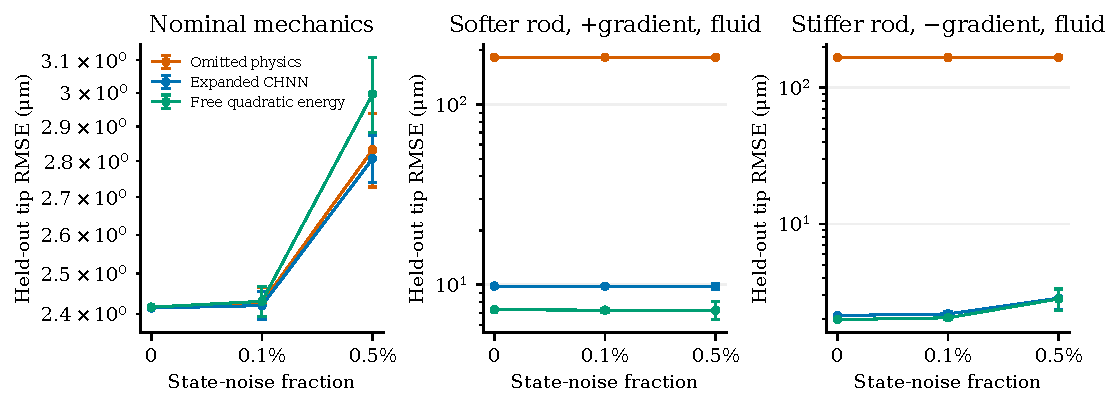
\includegraphics[width=\textwidth]{figures/robustness_noise_and_mismatch.pdf}
\caption{State noise and physics outside the nominal hypothesis class.
Each point averages three independent held-out trajectories. Bars show
the sample standard deviation across three training-noise seeds; the
clean fit is counted once. The higher-error model still re-identifies
its retained parameters.}
\label{fig:robustness-newphysics}
\end{figure*}

\subsection{Causal adaptation to slowly changing unknown parameters}
\label{sec:robustness-causal}
To test time variation separately from recalibration between settings,
we generate a $29$ s full-FE trajectory with a smooth drift. Define
$s=\operatorname{clip}_{[0,1]}((t-4\,\mathrm{s})/(24\,\mathrm{s}))$
and $a=(1-\cos\pi s)/2$. The hidden plant has
$e=0.85+0.20a$, $m=1.20-0.20a$ and
$\alpha/\alpha_{\rm ref}=1.40-0.40a$, while $G=0.5$ T/m and
$c_2=0.02$ kg/m$^2$ remain fixed. Multisine excitation continues
throughout. At cutoffs $8,12,16,20,24,28$ s, each estimator receives
only the preceding $4$ s of positions, velocities and known input.
It then predicts the next $1$ s from the currently observed state.
The coefficients are frozen before future state labels are accessed.

A constant sliding-window fit and a locally affine coefficient fit use
the same weak identity~\eqref{eq:robust-weakfit}; the latter adds features
multiplied by $(t-t_{\rm cut})/(4\,\mathrm{s})$. Linear constraints
preserve the nonnegative readouts over both the fitting interval and
the forecast interval. The known future input is supplied to all
predictors, but future states and true parameter values are withheld.
Across the six forecasts, the mean next-second tip RMSE is $387.483$
$\mu$m for the initial fit frozen at $4$ s, $59.217$ $\mu$m for causal
constant refitting and $9.867$ $\mu$m for causal affine adaptation.
The affine errors range from $2.701$ to $17.295$ $\mu$m. Constant
refitting is better at the final cutoff, where the physical drift
stops; this limitation of extrapolating a local trend is retained.
These are six forecasts on one declared drift trajectory, not independent
patient experiments or a general online-learning theorem.

\begin{figure}[t]
\centering
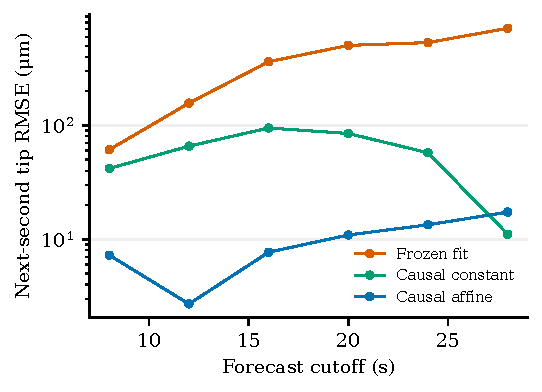
\includegraphics[width=\columnwidth]{figures/causal_parameter_adaptation.pdf}
\caption{One-second forecasts made using only past data under slow
material and magnetic drift. The frozen, constant and affine predictors
share the same current observed state and prescribed future input.}
\label{fig:causal-parameter-adaptation}
\end{figure}

For this nonautonomous plant, the physical energy ledger includes
$E_0[\dot e X^{\mathsf T}A_{\rm el}X/2+\dot m(1-\cos\vartheta)
-\dot g(G_{\rm ref}/B_0)(\ell^{\mathsf T}X)\sin\vartheta]$
in addition to magnetic input power and fluid losses. Its maximum
numerical residual is $6.06\times10^{-14}$ J. The stationary
conservative KAM certificates are not transferred to these driven,
dissipative, time-dependent trajectories.
